%this file is the second report
%a % comment anything after % until the end of the line

%minimum references to begin our article
\documentclass[12pt]{article}
\usepackage[english]{babel}
\usepackage[utf8]{inputenc}
\usepackage[T1]{fontenc}
\usepackage{graphicx}
\usepackage{fancyhdr}
\usepackage{hyperref}
\usepackage{float}
\usepackage{amsmath}
\usepackage[margin=1in]{geometry}
\usepackage{indentfirst}
\usepackage{titlesec}
\newcommand{\sectionbreak}{\clearpage}

\pagestyle{fancy}
%\cfoot{Fast and furious game playing: Monte Carlo drift}
% the last extension makes it possible to add images

%presentation of the document
\title{Fast and Furious Game Playing : Monte Carlo Drift\smallbreak Specifications report} %not sure about the name of this report
\author{Prateek \textsc{Bhatnagar}, Baptiste \textsc{Bignon}, \\
        Mikaïl \textsc{Demirdelen}, Gabriel \textsc{Prevosto}, \\
        Dan \textsc{Seeruttun-{}-Marie}, Benoît \textsc{Viguier} \\
        \\
        Supervisors: Nikolaos \textsc{Parlavantzas}, Christian \textsc{Raymond}}
\date{11/27/2014}
\setlength\parindent{15pt}
\begin{document}
\maketitle

\begin{figure}[!h] 
\centerline{\includegraphics[scale=0.50]{Pictures/arimaa}}
\end{figure}
\newpage


\begin{abstract}
%put abstract here
\end{abstract}
\newpage

%to add a table of contents
\tableofcontents
\newpage


\section{Introduction}					\label{sec:introduction}
\newpage

\section{General Architecture}				\label{sec:generalArchitecture}
	\subsection{Game behaviour}			\label{sec:gameBehavioiur}	In order to test the AI\footnote{Artificial Intelligence}, an application will be developped.
This application will include a two-player mode, a one-player mode and a demonstration mode (AI versus AI).
In the case where several AI have been implemented, the user will be able to choose which one to play against.

\begin{figure}[!h]
\centering
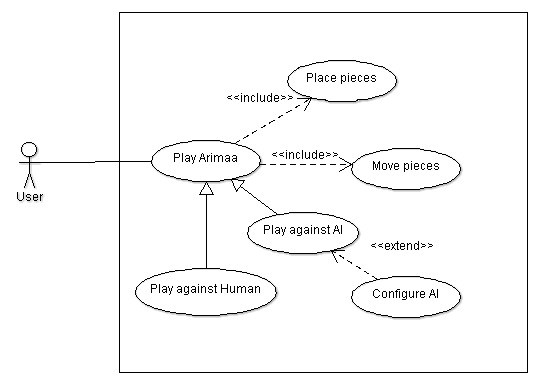
\includegraphics[width=\textwidth]{2General_Architecture/2.1Behaviour_of_the_Game/Pictures/Application_UCD}
\caption{The user-case diagram describing the application}
\label{fig:UCD_Play}
\end{figure}

In order to make the game easy to play, this application will provide a graphical User Interface (further referred to as \emph{UI}). % as described in part ??
This UI, as well as the algorithm for the AI, will act upon the game model, so as to inform it of what moves were made.
The UI will also regularly update to give the player feedback on the progression of the game.

	\subsection{Application-program interface}	\label{sec:api}
	\subsection{Inputs/Outputs}			\label{sec:io}
\newpage

\section{Algorithmic methods}				\label{sec:introduction}
	\subsection{Parallelization methods}		\label{sec:parallelization}		In order to increase the speed of our program, we have decided to parallelize it on a set of cluster of multicore machines. But there is many ways of parallelize our algorithm and we have to choose how we want to do it. 
\subsection{Previous Work}
In the last report, we talked about the different methods, their advantages and drawbacks. We have seen that there is mainly two parallelization methods that are efficient.
\newline
The first one is called the Root Parallelization. It consists in giving the tree to develop to every threads, let them develop it randomly without any communication with the environment
during a certain amount of time and then, merge the results of each tree.
This method has the great benefit of reducing at maximum the communication between the actors, in this case, the threads.
There's only a communication at the beginning and at the end, without needing any synchronization. The Root Parallelization is depicted in figure \ref{root}.
\newline
The other efficient parallelization method is called UCT-Treesplit. It looks like Root Parallelization as we give to each actor the same tree to develop.
Contrary to Root Parallelization, when the tree is develop on certain node, it goes on working packages who are distributed among every actor.
In terms of performance, this method is very efficient but need an High-Performance Computer, or HPC, and is very sensitive to network latency.
\newline
We have to choose two parallelization methods, one for the cluster parallelization and another for the shared memory parallelization.
\subsection{Cluster Parallelization}
For the cluster parallelization, we have to take into account the fact that we will need to communicate by sending messages, so it is relatively costly.
Moreover, as the network can have latency we should minimize the communication between the computers and that's why we have choose to implement a Root Parallelization.
It reduces the cost in communication at maximum, is very simple to implement,it does not depend of configuration of each computer and is very efficient.
\subsection{Shared Memory Parallelization}
For the shared memory parallelization we could choose both Root Parallelization or UCT-Treesplit.
If we choose UCT-Treesplit, we may not success to implement it correctly since it is a very complex strategy and, moreover, it may not be perfect BLA BLA BLA.

	\subsection{Monte Carlo tree search}		\label{sec:mcts}
\newpage

\section{Software solutions}				\label{sec:introduction}
	\subsection{OpenMP}				\label{sec:openmp}
	\subsection{OpenACC}				\label{sec:openacc}
	\subsection{MPI}					\label{sec:mpi}
\newpage

\section{Conclusion}					\label{sec:conclusion}		
The main focus area of this report is planning. Various planning methods have been decided such as Agile development methodology and Planning Poker method.
Using Agile Development Methodology, the incremental  development of the project will take place. Planning Poker method  which is the estimation technique of Agile Methodology is used to estimate the time requirement for the development of the project. The dates have been estimated with respect to the development of various models of our project.A serious attempt is made analyse the risks  in order to take preventive measures to avoid various risks and problems. 

\newpage

%uncomment to add bibliography
%\bibliography{bibliography}
%\bibliographystyle{plain}

\end{document}
